\begin{landscape}
\begin{table}[b]
%{
\fontsize{7.5}{9} \selectfont
\begin{tabular}{|l|l|l|l|l|l|l|l|l|}
\hline
 & \textbf{External Event} & \textbf{\begin{tabular}[c]{@{}l@{}}Random / \\ Conditional\end{tabular}} & \textbf{\begin{tabular}[c]{@{}l@{}}Influencing \\ factor\end{tabular}} & \textbf{\begin{tabular}[c]{@{}l@{}}Starting \\ Threshold\end{tabular}} & \textbf{\begin{tabular}[c]{@{}l@{}}Probability or\\ Preconditions\end{tabular}} & \textbf{\begin{tabular}[c]{@{}l@{}}Final \\ Threshold\end{tabular}} & \textbf{Impacted factor} & \textbf{Remarks} \\ \hline
\textbf{} & \textbf{Production \& Market:} & \textbf{} & \textbf{} & \textbf{} & \textbf{} & \textbf{} & \textbf{} &  \\ \hline
1 & \begin{tabular}[c]{@{}l@{}}Production problems \\ pop-up\end{tabular} & Conditional & \begin{tabular}[c]{@{}l@{}}production\\technology\end{tabular} & 2 & \begin{tabular}[c]{@{}l@{}}production \\ technology below 2 \end{tabular}& 1 & None, but Pop-Up & \\ \hline
2 & \begin{tabular}[c]{@{}l@{}}New technology \\ increases quality\end{tabular} & Conditional & \begin{tabular}[c]{@{}l@{}}baseQuality\end{tabular} & 80\% & $baseQuality^{3}$ &  100\% & cS & \begin{tabular}[c]{@{}l@{}}+30\% cS for 2 months\end{tabular} \\ \hline
3 & \begin{tabular}[c]{@{}l@{}}Company acquisition \\ possibility offered\end{tabular} & Conditional & \begin{tabular}[c]{@{}l@{}}Increasing \\ NOPAT\end{tabular} &  -  & \begin{tabular}[c]{@{}l@{}}NOPAT +30\% per \\ year over 5 years\end{tabular} &  -  & \begin{tabular}[c]{@{}l@{}}10000 cc added \\ to own company\end{tabular} & \begin{tabular}[c]{@{}l@{}}Acquisition costs \\ 70\% of current NOPAT, \end{tabular} \\ \hline
4 & \begin{tabular}[c]{@{}l@{}}Large company \\ overtakes market share\end{tabular} & Random &  -  &  -  & 0.02 &  -  & NOPAT - 10\% & \begin{tabular}[c]{@{}l@{}}Only possible if Net Worth \\ above 1mio cc\end{tabular} \\ \hline
5 & \begin{tabular}[c]{@{}l@{}}Company brand \\ reputation plunges\end{tabular} & Conditional & \begin{tabular}[c]{@{}l@{}}cS\end{tabular} &  20\%  & \begin{tabular}[c]{@{}l@{}}cS below 20\% \end{tabular} &  0\%  & cIS -20\% & Certain occurrence \\ \hline
6 & \begin{tabular}[c]{@{}l@{}}Computer virus attacks\end{tabular} & Random &  -  &  -  & 0.05 &  -  & \begin{tabular}[c]{@{}l@{}} pA - 50\% for \\ 3 months \end{tabular} & Only after year 2000 \\ \hline
\textbf{} & \textbf{Finance \& Taxes:} & \textbf{} & \textbf{} & \textbf{} & \textbf{} & \textbf{} & \textbf{} & {\color[HTML]{FE0000} } \\ \hline
7 & \begin{tabular}[c]{@{}l@{}}Tax changes lead to \\ higher or less rates\end{tabular} & Random &  -  &  -  & 0.05 &  -  & taxRate +/ 2\% & Changed for 1 year \\\hline
8 & Stricter eco laws & Conditional & \begin{tabular}[c]{@{}l@{}}ecoIndex\end{tabular} & 40\% & $ecoIndex^{0.31}-1$ & \begin{tabular}[c]{@{}l@{}}10\%  \\ \end{tabular} & \begin{tabular}[c]{@{}l@{}} 10\% NOPAT fine \\ Game Over at 10\% \end{tabular} & Shutdown by government \\ \hline
9 & Inflation changes & Random &  -  &  -  & \begin{tabular}[c]{@{}l@{}}0 to 2\% \\  \end{tabular} &  -  & NOPAT & NOPAT +/- 2\% \\ \hline
10 & \begin{tabular}[c]{@{}l@{}}Stealing inside of\\ the company\end{tabular} & Conditional & \begin{tabular}[c]{@{}l@{}} tJS\end{tabular} & 50\% & \begin{tabular}[c]{@{}l@{}}$\frac{0.2}{tJS}$\end{tabular} & 20\% & NOPAT & \begin{tabular}[c]{@{}l@{}}NOPAT -5000 cc \\ per employee \end{tabular} \\ \hline
\textbf{} & \textbf{Employees:} & \textbf{} & \textbf{} & \textbf{} & \textbf{} & \textbf{} & \textbf{} &  \\ \hline
11 & Strikes & Conditional & tJS & 10\% & $1-tJS^{0.7}$ & 0\% & \begin{tabular}[c]{@{}l@{}}  pDA- 80\%\end{tabular} & \begin{tabular}[c]{@{}l@{}}Only ends when \\ tJS above 10\end{tabular} \\ \hline
\textbf{} & \textbf{Natural disasters:} & \textbf{} & \textbf{} & \textbf{} & \textbf{} & \textbf{} & \textbf{} &  \\ \hline
12 & \begin{tabular}[c]{@{}l@{}}Flu goes around \\ causing ill employees\end{tabular} & Random &  -  &  -  & 0.1 &  -  & \begin{tabular}[c]{@{}l@{}}tEQoW - 10\%\end{tabular} & \begin{tabular}[c]{@{}l@{}}Duration 1 month \\ Only during winter\end{tabular} \\ \hline
13 & \begin{tabular}[c]{@{}l@{}}Hurricanes, tornadoes, \\ earthquakes\end{tabular} & Conditional & \begin{tabular}[c]{@{}l@{}}ecoIndex\end{tabular} & 40\% & $\frac{0.1}{ecoIndex}$ & 10\% &  cW - 2000 & Warehouse must be at 80\%\\ \hline
14 & \begin{tabular}[c]{@{}l@{}}Fire / Flooding in \\ warehouse\end{tabular} & Conditional & fSWH & \begin{tabular}[c]{@{}l@{}} 10\%\end{tabular} & $days \cdot 0.01$ & \begin{tabular}[c]{@{}l@{}} 10\%  \end{tabular} & sU - 30\% & \begin{tabular}[c]{@{}l@{}}Emptying warehouse \\ cancels event probability\end{tabular} \\ \hline
\textbf{} & \textbf{Government \& Politics:} & \textbf{} & \textbf{} & \textbf{} & \textbf{} & \textbf{} & \textbf{} &  \\ \hline
15 & \begin{tabular}[c]{@{}l@{}}Problems with customs \\ at the harbour\end{tabular} & Conditional & \begin{tabular}[c]{@{}l@{}}qSP\end{tabular} &   -  &  -  &  -  & Future work &  \\ \hline
16 & Change of power & Random &  -  &  -  &  -  &  -  & taxRate + 5\% & Most once per game \\ \hline
17 & \begin{tabular}[c]{@{}l@{}}Eco activists \\ block roads\end{tabular} & Conditional & tEIT &  30\%  &  -  &  0\%  & cF - 70\% & Active for 2 months\\ \hline
18 & \begin{tabular}[c]{@{}l@{}}Tensions between our \\ country and others\end{tabular} & Conditional & \begin{tabular}[c]{@{}l@{}}Change \\ of power\end{tabular} &  -  &  -  &  -  & Future Work &  \\ \hline
\end{tabular}
    \caption{External events overview}
    \label{events_list}
\end{table}
\end{landscape}


\begin{figure}
    \centering
    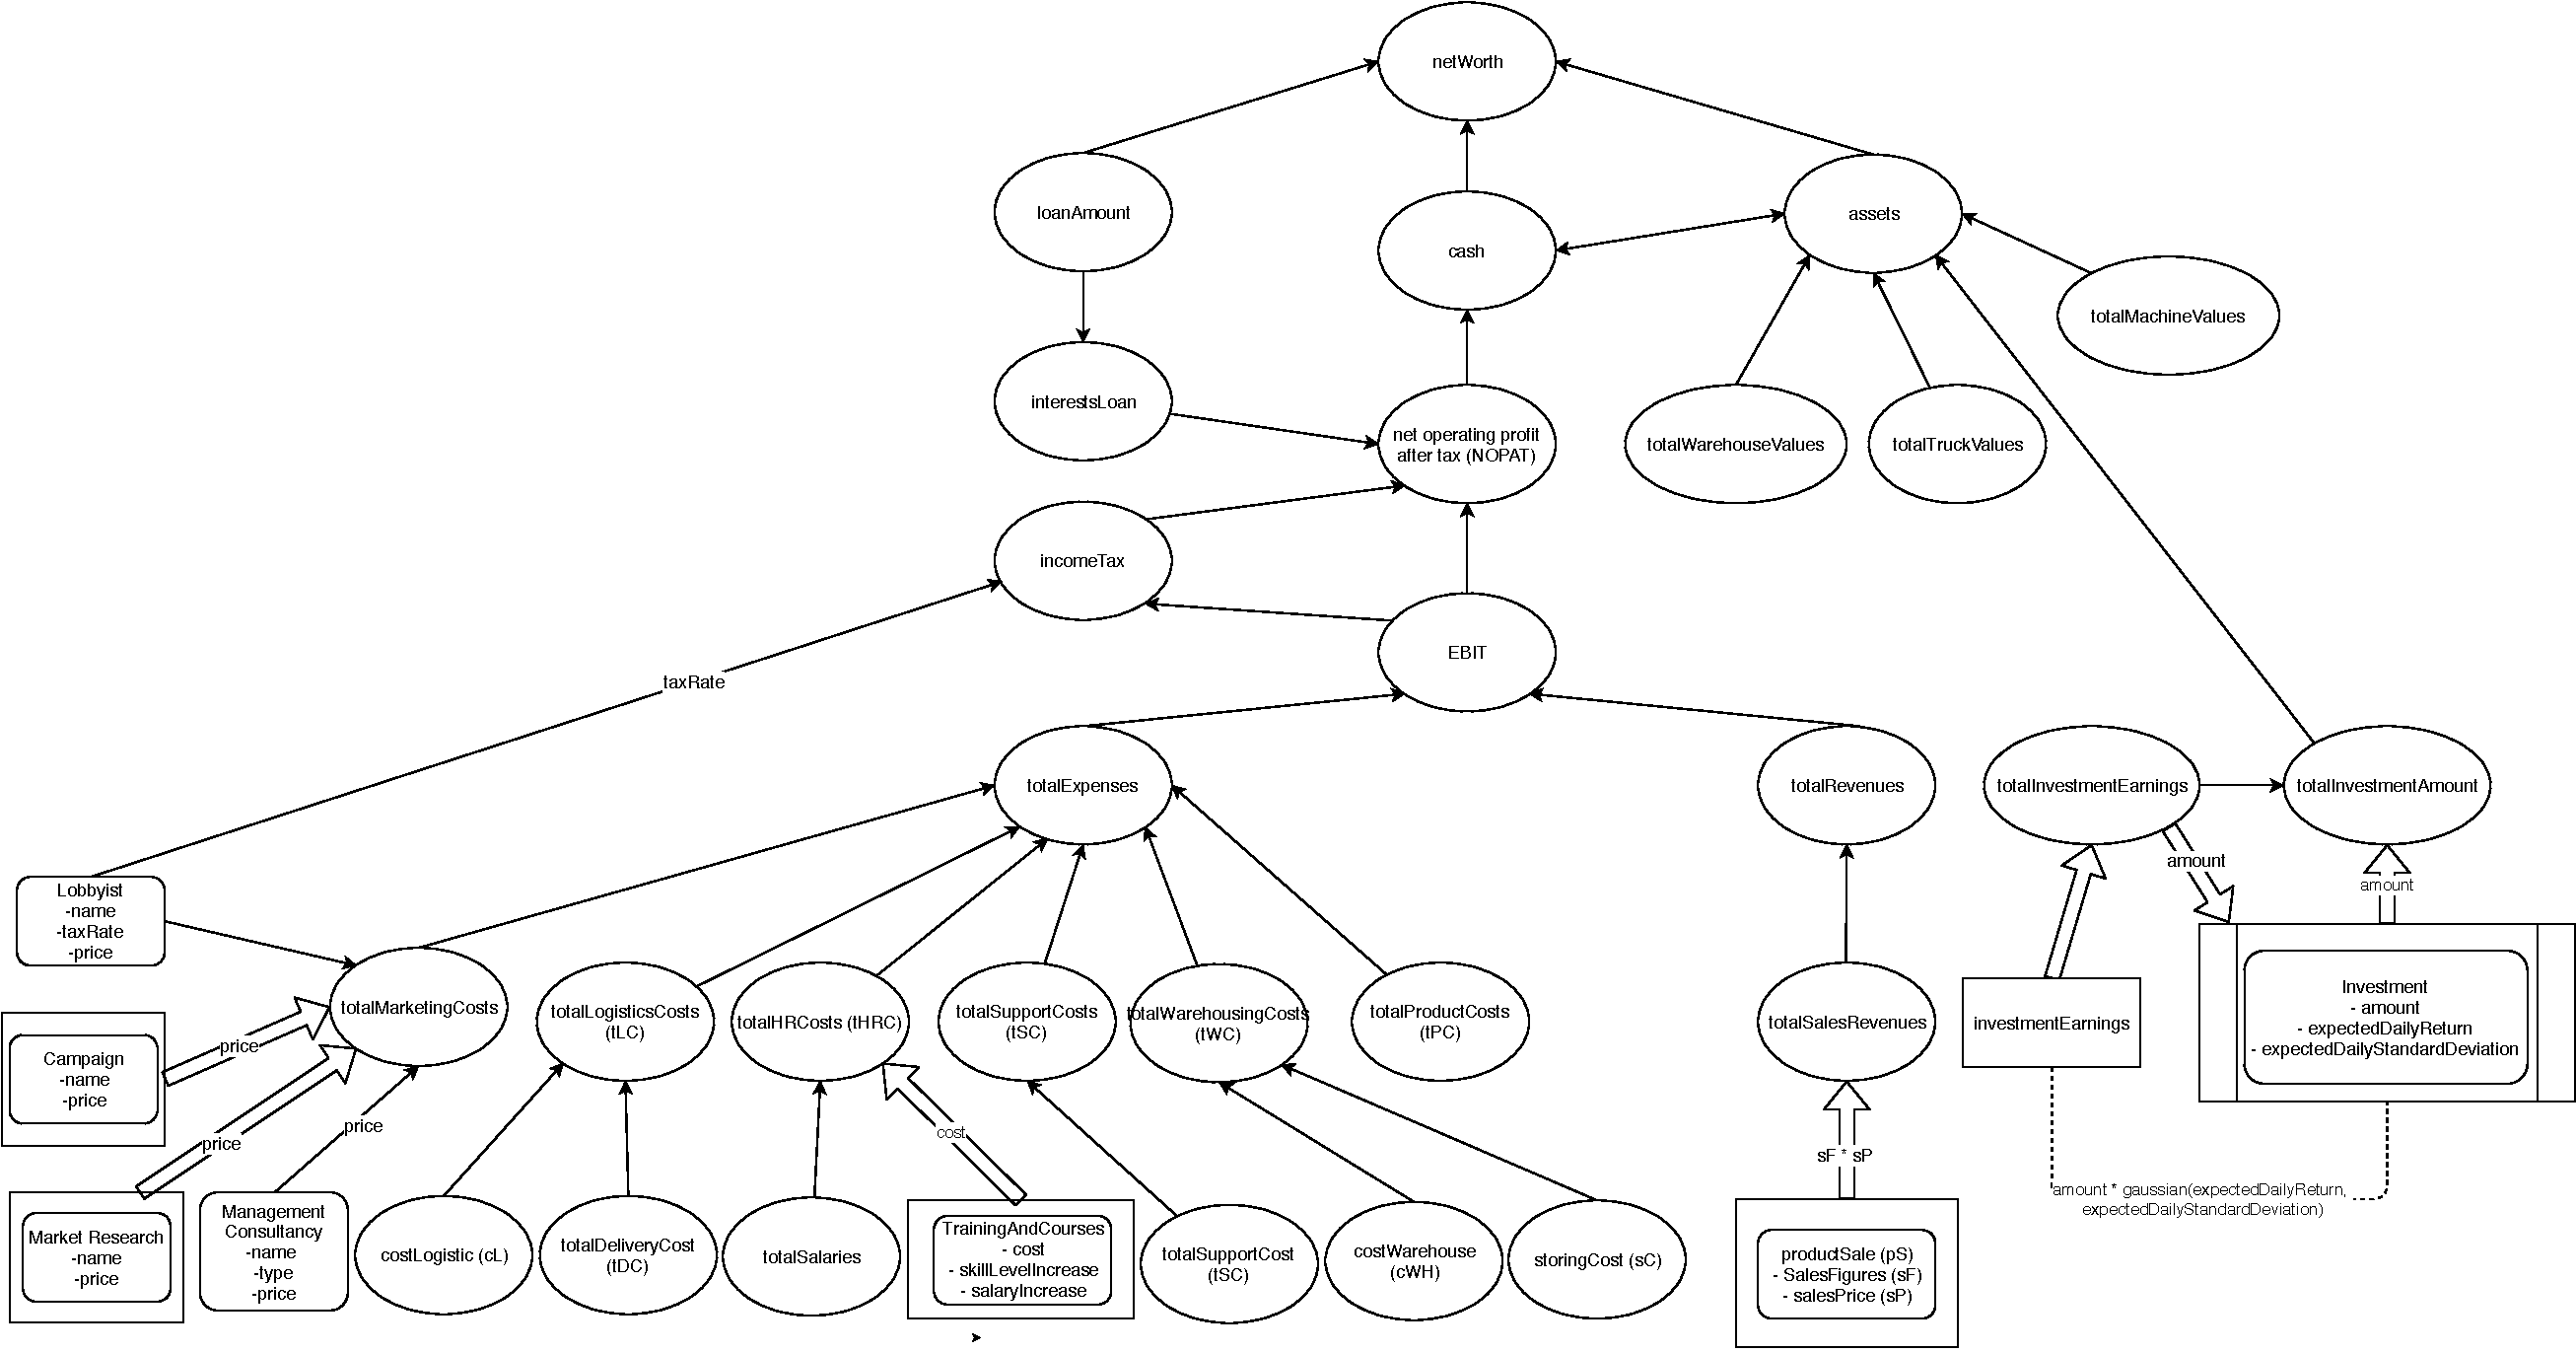
\includegraphics [angle=90, scale=0.4]{financeGraph.pdf}
    \caption{Finance Graph}
    \label{fig:finance_graph}
\end{figure}

\begin{figure}
    
\includegraphics [scale=0.3]{images/loanDenied.png}
    \caption{UI loan denied by bank}
    \label{fig:loan_denied}
\end{figure}

\begin{figure}
    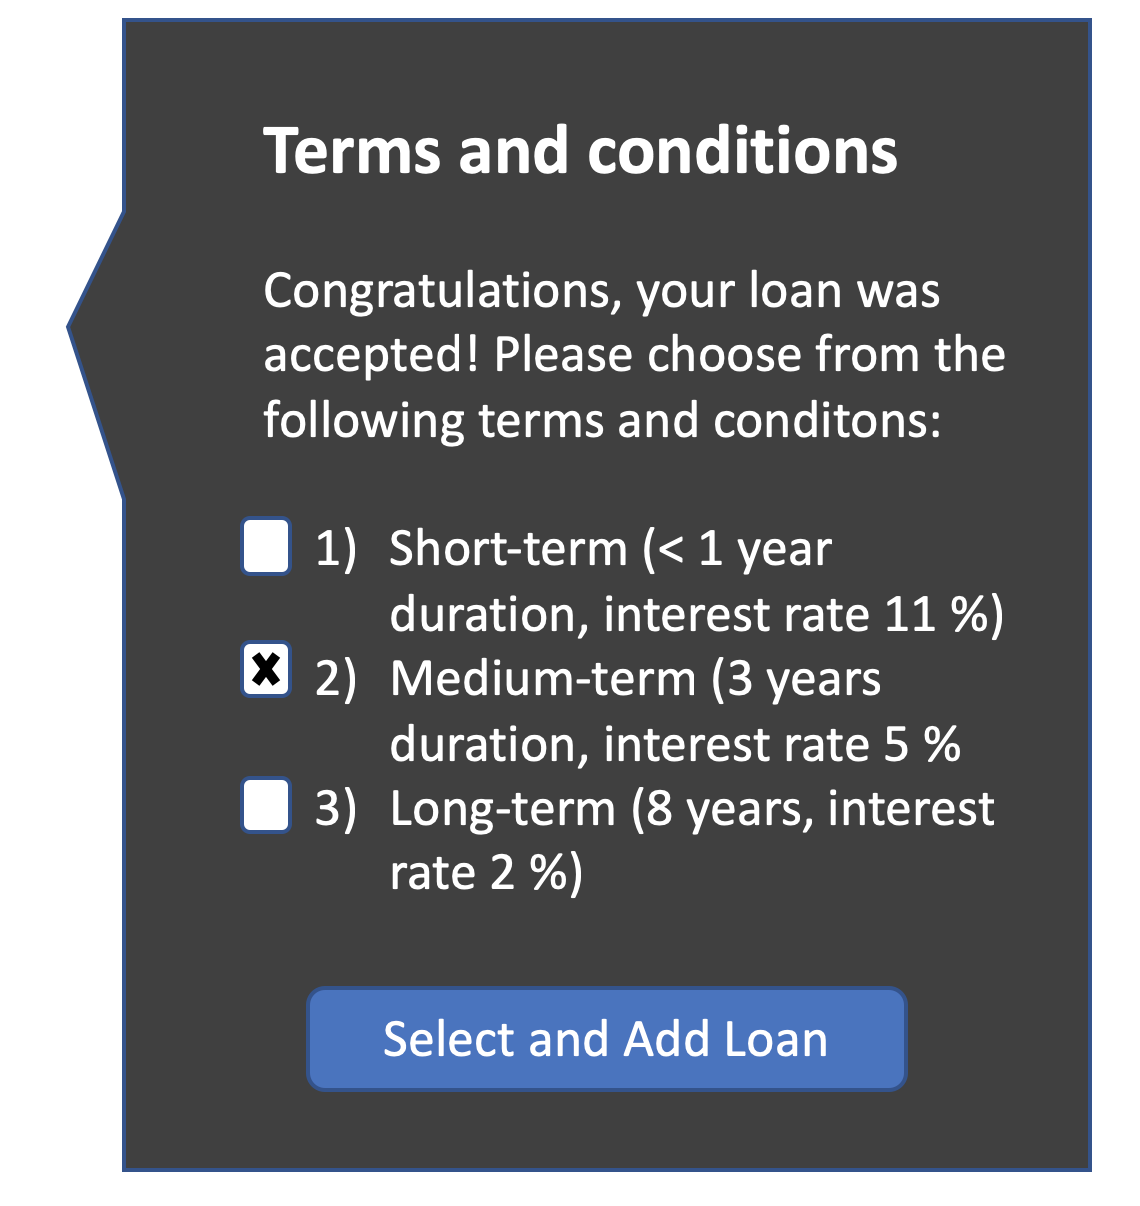
\includegraphics[scale=0.3]{images/loanAccepted.png}
    \caption{UI loan accepted by bank}
    \label{fig:loanAccepted}
\end{figure}

\begin{figure}
    \centering
    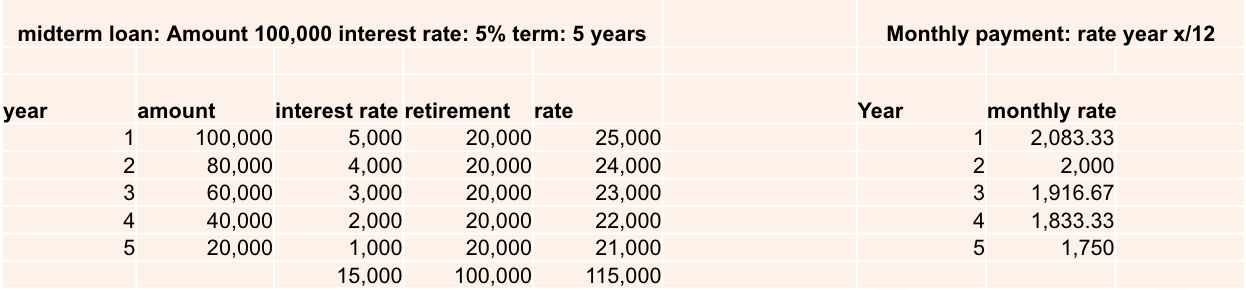
\includegraphics[width=\textwidth]{images/loanRepayment.png}
    \caption{Loan repayment model example}
    \label{fig:loanRepayment}
\end{figure}